\section{LoRa}\label{sec:etat_art-lora}
\renewcommand{\rightmark}{LoRa}

LoRa (Long Range) est une technologie radio  fonctionnant sur une modulation radio propriétaire
détenue par Semtech. Cette modulation est dérive de la modulation \textit{chirp spread spectrum (CSS)} et permet d'obtenir des communications longues portées et basses énergie.
%todo chiffres

\begin{wrapfigure}{r}{0.3\textwidth}
    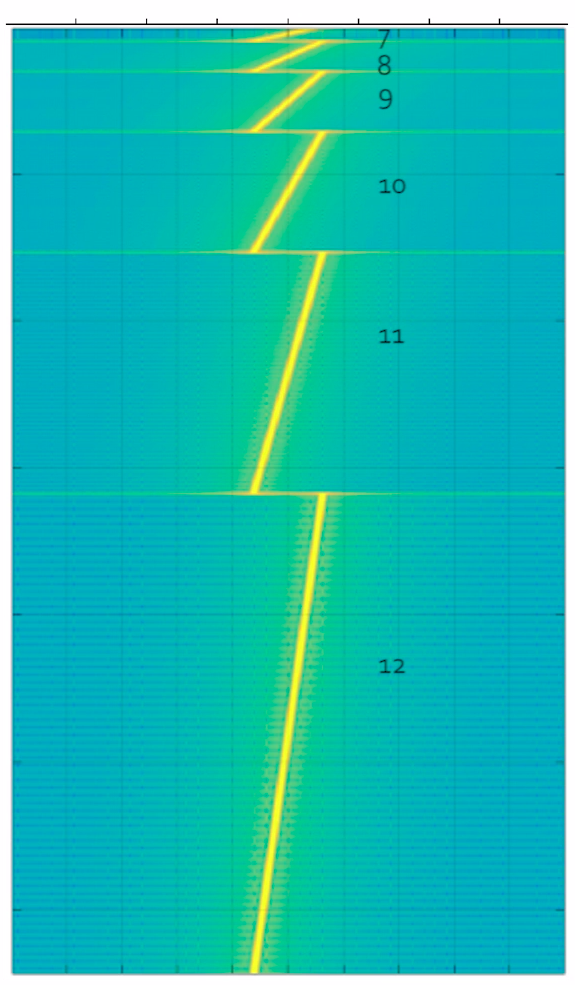
\includegraphics[scale=0.25]{res/pictures/lora-sf.png}
    \caption{Signal en fonction du SF.\todo{ref}}
    \label{fig:state-sf}
\end{wrapfigure}
Une communication LoRa dépend des paramètres suivants:
\begin{itemize}
    \item \textbf{Spreading Factor (SF)}: SF est une variable qui définit la vitesse de balayage du signal radio (Fig~\ref{fig:state-sf}). Le spreading factor est compris entre 7 et 12. Plus la valeur est grande, plus la vitesse de balayage est petite et donc le signal est plus facile à décoder. mais le débit des données est plus faible. Donc une grande valeur de SF implique un débit plus faible mais une QoS (Quality of Service) plus élevée et inversemment pour une petite valeur de SF.
    \item \textbf{Bandwidth (BW)}: Détermine la largeur de la bande passante. Une bande passante plus large augmente la qualité du signal. Pour LoRa, en Europe, les valeurs de BW sont limitées à 125 KHz et 250KHz.\todo{ref thethingsnetwork}
    \item \textbf{Coding rate (CR)}:D'après \todo{ref}, LoRa utilise FEC (Forward error correction) pour chaque transmission. L'uilisation de cette méthode de correction d'erreur utilisant la redondance permet au signal de supporter de courtes interférences. Ainsi il possible de coder des données de 4 bits avec des redondances de 5, 6, 7 ou 8 bits. La valeur du CR se note donc 
    4/5, 4/6, 4/5 ou 4/8.
    %https://josefmtd.com/2018/08/14/spreading-factor-bandwidth-coding-rate-and-bit-rate-in-lora-english/
\end{itemize}

La relation entre SF et BW est décrite par l'équation~\ref{eq:state-lora-rs}.
\begin{equation}\label{eq:state-lora-rs}
    Rs = \frac{BW}{2^{SF}}
\end{equation}

\vspace{1cm}
Le format des paquets LoRa(Fig.~\ref{fig:state-lora-frame-format}) peut être explicite ou implicite.
Dans le mode implicite, le header n'est pas inclus dans le paquet. Pour cela, la taille de la payload, le coding rate et la présence de la Payload CRC doit être configuré.
Ce mode permet de réduire la taille du paquet et donc du temps de transmission.

\begin{figure}[H]
    \centering
    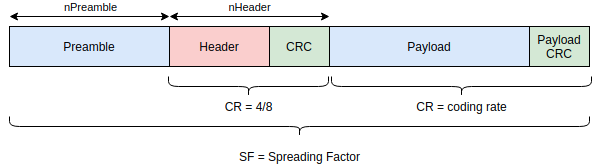
\includegraphics[scale=0.6]{res/pictures/lora-frame-format.drawio.png}
    \caption{Format d'un paquet LoRa.}
    \label{fig:state-lora-frame-format}
\end{figure}

Le temps d'émission d'un paquet LoRa est défini par l'équation~\ref{eq:state-lora-tframe}.
\begin{equation}\label{eq:state-lora-tframe}
    T_{frame} = T_{preamble} + T_{payload}
\end{equation}

Où $T_{preamble}$ et $T_{payload}$ sont respectivement le temps d'émission du preamble et du payload définis aux équations \ref{eq:state-lora-tpreamble} et \ref{eq:state-lora-tpayload}.

\begin{equation}\label{eq:state-lora-tpreamble}
    T_{preamble} = (n_{preamble} + 4,25)T_{sym}
\end{equation}

\begin{equation}\label{eq:state-lora-tpayload}
    T_{payload} = n_{payload} * T_{sym}
\end{equation}

Où $T_{sym} = \frac{1}{R_s}$, $n_{preamble}$ et $n_{payload}$ sont le nombre de symboles du preamble et du payload. $n_{preamble}$ est une valeur définie dans le module radio et $n_{payload}$ est défini par l'équation~\ref{eq:state-lora-npayload}.

\begin{equation}\label{eq:state-lora-npayload}
    \begin{split}
    n_{payload} =8 +max
     \left( ceil \left[ \frac{8PL - 4SF + 28 + 16CRC - 20IH}{4(SF-2DE)} \right] (CR+4), 0 \right)
    \end{split}
\end{equation}

où:
\begin{itemize}
    \item $PL$ est le nombre d'octets de la payload (1 à 255)
    \item $IH=0$ si le header est présent, $IH=1$ sinon
    \item $DE=1$ si $LowDataRateOptimize=1$, $DE=0$ sinon
    \item $CR$ prend la valeur 1 pour $4/5$, 2 pour $4/6$, etc
\end{itemize}
